\documentclass[journal,twoside]{IEEEtran}
\usepackage{preamble}
\usepackage{pbalance}

\markboth{Southeast University Software-Defined Radio Experiment Course, January 2024}{W. Zhao: Dual-Mode PSK Transceiver on SDR With FPGA}
\IEEEpubid{
  \begin{tabular}[t]{c}
    \copyright{} 2024 Wuqiong Zhao.
    This work is licensed under a Creative Commons Attribution-ShareAlike 4.0 License.\\
    For more information, see \url{https://creativecommons.org/licenses/by-sa/4.0/}.
  \end{tabular}
}

\hypersetup{
  , pdftitle    = {Dual-Mode {PSK} Transceiver on {SDR} With {FPGA}}
  , pdfauthor   = {Wuqiong Zhao}
  , pdfsubject  = {Southeast University Software-Defined Radio Experiment Course}
  , pdfkeywords = {Phase-shift keying (PSK), software-defined radio (SDR), transceiver design, modulation, demodulation, field programmable gate array (FPGA).}
}

\begin{document}

  \title{Dual-Mode PSK Transceiver on SDR With FPGA}

  \author{%
    Wuqiong~Zhao{\hspace{.1em}\textsuperscript{\orcidicon{0000-0002-9550-7423}}},~\IEEEmembership{Student Member, IEEE}
    \thanks{Date of publication 16 January 2024; date of current version 17 January 2024.
      The author would like to thank Lecturer Dan Yang for the guidance and help in the course of the experiment.
      The author would also like to thank AI tools including GitHub Copilot and Claude.AI for their help in preparing this paper.}
    \thanks{Wuqiong Zhao is with Southeast University, Nanjing 211189, China. (e-mail: wqzhao@seu.edu.cn, website: \url{https://wqzhao.org}).}
    \thanks{Online URL: \url{https://go.wqzhao.org/sdr-psk-fpga}}
    % \vspace{-1mm}
  }

  \maketitle

  \begin{abstract}
    In this experiment, we implement a dual-mode PSK transceiver on SDR with FPGA,
    supporting both BPSK and QPSK.
    Moreover, the transceiver is designed to be able to switch between the two modes by introducing a packet-based communication protocol,
    where modulation information can be extracted from the packet header.
    The design is resource-efficient implemented using block diagrams with intellectual property (IP) cores and Verilog modules in Vivado.
    Both simulation results and experiment observations on an SDR platform verify the effectiveness of the design.
  \end{abstract}
  \begin{IEEEkeywords}
    Phase-shift keying (PSK), software-defined radio (SDR), transceiver design, modulation, demodulation, field programmable gate array (FPGA).
  \end{IEEEkeywords}

  \section{Introduction}

    \IEEEPARstart{S}{oftware-defined} radio (SDR) is useful in various applications,
    including rapid prototyping and research.
    A millimeter wave (mmWave) SDR platform \cite{zhao2020m} can enable research in both mmWave physical-layer communications
    and the high-level networking problems.
    %
    Phase-shift keying (PSK) is a popular modulation scheme in digital communications.
    Among PSK, the simplest two are the binary PSK (BPSK) and the quadrature PSK (QPSK).
    The carrier extraction is required for coherent demodulation,
    though differential encoding can be used to avoid the carrier extraction.
    %
    Field programmable gate array (FPGA) is a popular choice for SDR baseband processing,
    due to its flexibility and high performance.
    In this project,
    instead of employing high-level synthesis (HLS) \cite{zhao2023flexible},
    we directly implement the transceiver on FPGA using hardware description language (HDL) Verilog,
    for better control of the underlying hardware and a more efficient design.

    To benefit the research and learning community,
    the design sources (Vivado project) and this paper (in \LaTeX) are open source \cite{github_repo}.
    %
    The contributions of this paper is summarized as follows:
    \begin{enumerate}
      \item We implement a dual-mode PSK transceiver on SDR with FPGA, enabling both BPSK/QPSK modulation and coherent demodulation,
      with carrier synchronization and symbol synchronization.
      \item A packet-based communication is introduced to enable the switching between BPSK and QPSK based on header fields,
      another step towards to a flexible and ready-to-use transceiver.
      \item The open-source design is implemented on a Zynq-7020 FPGA and verified on an SDR platform, demonstrating its effectiveness.
    \end{enumerate}

  \section{System Overview}

    \subsection{Software-Defined Radio}

      We employ eNodeX 30B \cite{eNodeX}, an SDR platform equipped with a pair of
      configurable Global System for Mobile Communications (GSM) transmitter (Tx) and receiver (Rx) antennas.
      An MS Windows software is provided for configurations,
      including the sampling frequency, the carrier frequency, attenuation and gain, etc.

    \subsection{Transceiver Design}

      The current transmitter and receiver are implemented on the same FPGA,
      but the implementation can be readily extended for different FPGAs with small frequency offsets.
      The system overview is shown in Fig.~\ref{fig:system_overview}.
      \begin{figure}[htbp]
        \centering
        \begin{tikzpicture}[
  , thick
  , n/.style = {
    , draw
    , fill = myblued!15
    , align = center
  }
  , font = \small\sffamily
]
  \node [n] {RF Data\\Converter};
\end{tikzpicture}%

        \caption{Transceiver system overview.}
        \label{fig:system_overview}
      \end{figure}

      \IEEEpubidadjcol
      \textbf{Clock Generator}.
      Required clocks are generated from the programmable logic (PL) clock.
      All reset signals are generated using Processor System Reset Modules \cite{xilinx:pg164},
      which can provide synchronized power-up reset signals.

      \textbf{RF Data Converter}.
      This block contains analog-to-digital converters (ADCs) and digital-to-analog converters (DACs),
      enabled by a vendored AD9361 module \cite{ad9361}.

      \textbf{Tx Signal Generator}.
      The transmitted signal is generated in this block.
      Currently, it repeats a certain pattern and does not accept external input.
      But it can be readily extended to a more complicated design, based on the current interface template.

      \textbf{Rx Processor}.
      This block is responsible for processing the received signal,
      including demodulation and data extraction from a packet.
      It is the most complex (and the core) block in the system.

      \textbf{System ILA}.
      The system integrated logic analyzer (system ILA) \cite{xilinx:pg261} is used to observe the internal signals.

      \textbf{Constant Configurations}.
      Several parameters can be configured in this block.
      Most importantly, the mode control constants (\texttt{MODE\_CTRL}) are shown in Table~\ref{tab:mode_ctrl}.
      \begin{table}[htbp]
        \caption{Mode Control Constants}
        \label{tab:mode_ctrl}
        \renewcommand{\arraystretch}{1.2}
        \rowcolors{1}{white}{gray!15}
        \begin{tabularx}{\linewidth}{cYYYc}
          \toprule\tabvertspace
          \textbf{Mode} & \textbf{Localparam} & \textbf{Value} & \textbf{\ttfamily is\_bpsk} & \textbf{Packet} \\
          \tabvertspace\midrule
            BPSK & \texttt{MODE\_BPSK} & \texttt{4\textquotesingle b0001} (1) & \texttt{1\textquotesingle b1} & No \\
            QPSK & \texttt{MODE\_QPSK} & \texttt{4\textquotesingle b0010} (2) & \texttt{1\textquotesingle b0} & No \\
            Mixed & \texttt{MODE\_MIX~~} & \texttt{4\textquotesingle b0100} (4) & variable & Yes \\
          \bottomrule
        \end{tabularx}
      \end{table}

      % As shown in Table~\ref{tab:mode_ctrl},
      The system can be configured to work in BPSK, QPSK, or the mixed mode.
      The remaining part of the paper will focus on the mixed mode,
      which has \texttt{MODE\_CTRL} equal to \texttt{MODE\_MIX} (\texttt{4\textquotesingle b0100})
      and has a packet-based communication.
      Details of the design of packets are in Section~\ref{sec:packet-based}.

    \subsection{BPSK/QPSK Modulation}\label{subsec:modulation}

      The BPSK and QPSK modulation constellation graphs used in the system are shown in Fig.~\ref{fig:constellation}.
      Different from the traditional setting, out adopted BPSK constellation in Fig.~\subref*{subfig:constellation_BPSK}
      is a combination of in-phase (I) and quadrature (Q) components.
      This is to make sure the phases used in BPSK are among those in QPSK,
      enabling a smooth transition between the two modes,
      which is critical because the header field is always modulated in BPSK.
      The QPSK constellation in Fig.~\subref*{subfig:constellation_QPSK} satisfies the Gray code:
      two adjacent values in the constellation differ in only one bit.
      \begin{figure}[htbp]
        \subfloat[BPSK.\label{subfig:constellation_BPSK}]{\begin{tikzpicture}[
  , thick
  , axis/.style = {
    , -latex
  }
  , n/.style = {
    , circle
    , fill = myblued
    , inner sep = 0pt
    , minimum size = 4pt
  }
  , l/.style = {
    , dotted
  }
  , ll/.style = {
    , dashed
    , myred
    , shorten < = -8pt
    , shorten > = -8pt
  }
  , outer sep = 0
  , inner sep = 2pt
]
  \draw [axis] (-1.5, 0) -- (1.5, 0) [right] node {$I\,(\cos)$};
  \draw [axis] (0, -1.5) -- (0, 1.5) [above] node {$Q\,(\sin)$};
  \draw [ll] (-1, 1) -- (1, -1);
  \draw [l] (0, 1) -- (1, 1);
  \draw [l] (0, -1) -- (-1, -1);
  \draw [l] (1, 0) -- (1, 1);
  \draw [l] (-1, 0) -- (-1, -1);
  \node [n, label={right:\ttfamily\bfseries0}] at (1, 1) {};
  \node [n, label={left:\ttfamily\bfseries1}] at (-1, -1) {};
\end{tikzpicture}%
}\hfill%
        \subfloat[QPSK.\label{subfig:constellation_QPSK}]{\begin{tikzpicture}[
  , thick
  , axis/.style = {
    , -latex
  }
  , n/.style = {
    , circle
    , fill = myblued
    , inner sep = 0pt
    , minimum size = 4pt
  }
  , l/.style = {
    , dotted
  }
  , ll/.style = {
    , dashed
    , myred
    , shorten < = -8pt
    , shorten > = -8pt
  }
  , outer sep = 0
  , inner sep = 2pt
]
  \draw [axis] (-1.5, 0) -- (1.5, 0) [right] node {$I\,(\cos)$};
  \draw [axis] (0, -1.5) -- (0, 1.5) [above] node {$Q\,(\sin)$};
  \draw [l] (-1, 1) -- (1, 1);
  \draw [l] (1, -1) -- (-1, -1);
  \draw [l] (1, -1) -- (1, 1);
  \draw [l] (-1, 1) -- (-1, -1);
  \node [n, label={right:\ttfamily\bfseries00}] at (1, 1) {};
  \node [n, label={below:\ttfamily\bfseries01}] at (1, -1) {};
  \node [n, label={left:\ttfamily\bfseries11}] at (-1, -1) {};
  \node [n, label={above:\ttfamily\bfseries10}] at (-1, 1) {};
\end{tikzpicture}%
}%
        \caption{BPSK/QPSK modulation constellation used in the system.}
        \label{fig:constellation}
      \end{figure}

      The design heavily relies on the \textbf{a}dvanced e\textbf{x}tensible \textbf{i}nterface (AXI) \cite{xilinx:ug1037},
      and the AXI stream (AXIS) protocol is used for data transmission,
      which requires the data width is a multiple of 8 bits (1 byte) in Vivado.
      Therefore, we define the BPSK uses bit 1, and QPSK uses bits 1 and 0,
      both counting from the least significant bit (LSB).

    \section{Transmitter}

    \subsection{Carrier NCO}

      The carrier frequency is generated by a numerically controlled oscillator (NCO).
      In Vivado, we use the Direct Digital Synthesis (DDS) Compiler IP \cite{xilinx:pg141} as the NCO.
      Both the cosine and sine components are used.
      Due to the need of carrier synchronization (see Section~\ref{subsec:costas}),
      the DDS does not have a fixed frequency,
      but an input stream signal controlling the phase,
      connected from the module \texttt{NCO\_Phase} (see Eq.~\eqref{eq:Tx_NCO}).

  \subsection{PSK Modulation}

    \subsubsection{Pseudo-random Number (PN) Generator}

      In this experiment, the transmitted signal are pseudo-random number (PN) sequences.
      Typically, we implement the PN generator with $N=4$ (period is $2^4-1=15$) and $N=5$ (period is $2^5-1=31$)
      using a shift register \cite{james1990review}.
      Thus, the 2-bits signal aggregating the I and Q components has the period of $465$.
      The Verilog code for the module \texttt{PN\_Gen} is shown below.
      \begin{minted}[highlightlines={11,18}]{verilog}
module PN_Gen # (parameter N = 5) (
  input      clk,
  output reg pn
);
  reg [N-1:0] PN_buf = 1; wire rst;
  generate
  if (N == 5)
    always @ (posedge clk)
      if (rst) begin PN_buf <= 5'd1; pn <= 0; end
      else begin
        PN_buf <= { PN_buf[3:0], PN_buf[4] ^ PN_buf[2] };
        pn <= PN_buf[4];
      end
  else if (N == 4)
    always @ (posedge clk)
      if (rst) begin PN_buf <= 4'd1; pn <= 0; end
      else begin
        PN_buf <= { PN_buf[2:0], PN_buf[3] + PN_buf[2] };
        pn <= PN_buf[3];
      end
  else ; // NOT implemented yet!
  endgenerate
  assign rst = !(|PN_buf);  // reset when PN_buf is all 0
endmodule
      \end{minted}

    \subsubsection{Modulation With I and Q Streams}

      The modulation is performed by selecting the appropriate carrier phase
      according to the input bits and the constellation (in Fig.~\ref{fig:constellation}).
      Note the Q component is always $90^\circ$ ahead of the I component.
      The modulated I and Q components are then connected to the corresponding DAC ports.

  \section{Receiver}

    \subsection{Overview}

      The receiver performs carrier synchronization, symbol synchronization and PSK detection first,
      without considering the packet structure.
      The depacketizer and the packet extraction is based on the synchronized bit stream after PSK detection.

    \subsection{Carrier Synchronization Using Costas Loop}\label{subsec:costas}

      A Costas loop \cite{simon1977optimum} is used for carrier synchronization.
      The basic idea of a Costas loop is to provide an error (carrier phase offset) feedback.
      The negative feedback is used to lock the carrier phase to the PSK signal.
      The generation of the error feedback is specific to different modulation schemes,
      as well as their constellation graphs.

      The proposed dual-mode Costas loop is shown in Fig.~\ref{fig:costas_loop},
      which can be switched between BPSK and QPSK via a control signal \texttt{is\_bpsk}.
      The two multipliers directly following the PSK stream input are phase detectors,
      whose low-frequency components represent the data stream signal.
      Therefore, the data stream I and Q signal can be extracted after passing the mixed signals through a low-pass filter (LPF).
      Thus, it is ready to map the obtained I/Q signal to the constellation graph,
      and generate the error signal.
      \begin{figure}[htbp]
        \centering
        \begin{tikzpicture}[
  , thick
  , font = \small\sffamily
  , node distance = 8mm and 5mm
  , 1bit/.style = {
    , semithick
  }
  , font xs/.style = {
    , font = \notsotiny\sffamily
  }
  , n/.style = {
    , draw
    , minimum height = 5mm
    , fill = #1!15
  }
  , n/.default = myblued
  , LPF/.style = {
    , n = myyellow
    , minimum width = 6mm
  }
  , arr/.style = {
    , -latex
  }
  , arr r/.style = {
    , latex-
  }
  , port/.style = {
    , n = gray
    , signal
    , signal to = east
    , minimum height = 2mm
  }
  , port label/.style = {
    , font xs
    , align = center
    , below = 1mm
  }
  , mul add base/.style = {
    , draw = black
    , circle
    , minimum width = 3mm
    , fill = none
  }
  , add/.style = {
    , mul add base
    , append after command = {
      \pgfextra
        \draw [-, black] (\tikzlastnode.north) -- (\tikzlastnode.south);
        \draw [-, black] (\tikzlastnode.east)  -- (\tikzlastnode.west);
      \endpgfextra
    }
  }
  , sub/.style = {
    , mul add base
    , append after command = {
      \pgfextra
        \draw [-, black] (\tikzlastnode.north) -- (\tikzlastnode.south);
        \draw [-, black] (\tikzlastnode.east)  -- (\tikzlastnode.west);
        \node [above left = 0mm and 0mm of \tikzlastnode.north, inner sep = 0] {\notsotiny\resizebox*{\widthof{+}}{\heightof{-}}{-}};
        \node [above right = 0mm and 0mm of \tikzlastnode.east, inner sep = 0] {\notsotiny+};
      \endpgfextra
    }
  }
  , mul/.style = {
    , mul add base
    , append after command = {
      \pgfextra
        \draw [-, black] (\tikzlastnode.north west) -- (\tikzlastnode.south east);
        \draw [-, black] (\tikzlastnode.north east) -- (\tikzlastnode.south west);
      \endpgfextra
    }
  }
  , null node/.style = {
    , inner sep = 0
    , outer sep = 0
    , minimum width = 0
    , 
  }
  , joint/.style = {
    , circle
    , minimum height = 0.8mm
    , inner sep = 0
    , fill = #1
    , draw = #1
  }
  , joint/.default = black
  , mux/.style = {
    , n = mygreen
    , trapezium
    , trapezium angle = 60
    , shape border rotate = 90
    , minimum height = 3.8mm
    , anchor = south
  }
]
  \node (nco) [n] {NCO};
  \node (loop-filter) [LPF, right = of nco] {};

  \node (lpf-I) [LPF, above = of loop-filter] {};
  \node (lpf-Q) [LPF, below = of loop-filter] {};

  \node (mul-I) [mul, xshift = -7mm] at (nco |- lpf-I) {};
  \node (mul-Q) [mul, xshift = -7mm] at (nco |- lpf-Q) {};

  \node (in-j) [joint, left = 8mm of nco] {};
  
  \draw [arr] (loop-filter) -- (nco);
  \draw [arr] ([yshift = +1mm]nco.west) -| (mul-I) node [midway, right, yshift = +7mm] {$\cos$};
  \draw [arr] ([yshift = -1mm]nco.west) -| (mul-Q) node [midway, right, yshift = -7mm] {$\sin$};

  % input port
  \draw (in-j) -- ++ (-6mm, 0) node [port] {}
                               node (in-psk) [port label] {PSK\\strm.};

  % mux
  \draw [arr r] (loop-filter.east) -- ++ (5mm, 0) node (mux) [mux, right] {}
                                                  node [font xs, above right = .5mm and 1.2mm, inner sep = 0] {0}
                                                  node [font xs, below right = .5mm and 1.2mm, inner sep = 0] {1};
  \draw [1bit, shorten < = -.1mm] (mux.north)
    to [jump, jump pos = .595, |u-, jump swap] ([yshift = 5mm] in-psk |- mul-I.north) node [port] {}
                                                                                      node [port label] {is\_bpsk};

  % error output
  \node [sub, right = of mux.east, yshift = +2.2mm] (sub-QPSK) {};
  \draw [arr] (sub-QPSK) -- (sub-QPSK.west -| mux.east);
  \node [mul, right = of mux.east, yshift = -2.2mm] (mul-BPSK) {};
  \draw [arr] (mul-BPSK) -- (mul-BPSK.west -| mux.east);

  % error detector
  \node (err-detect-ctrl) [n = myred, align = center, anchor = west] at ([xshift = 10mm] mul-BPSK.east |- loop-filter.east) {Error\\Detector\\Control};
  \draw (sub-QPSK) -- (sub-QPSK -| err-detect-ctrl.west) node [above left, font xs, inner sep = .5mm, align = center] {\hphantom{Q}\\I};
  \draw (mul-BPSK) -- (mul-BPSK -| err-detect-ctrl.west) node [above left, font xs, inner sep = .5mm] {Q};
  \draw ([xshift = -3.5mm] sub-QPSK-| err-detect-ctrl.west) node [joint] {} to[jump, jump pos = .55] ++ (0, -8mm) -| (mul-BPSK);
  \draw ([xshift = -6.5mm] mul-BPSK-| err-detect-ctrl.west) node [joint] {} to[jump, jump pos = .55, jump swap] ++ (0, +8mm) -| (sub-QPSK);
  \node (err-detect) [fit = (err-detect-ctrl) (mux), draw, dashed, myred] {};
  \node [myred, anchor = north west, inner xsep = 0] at (err-detect.south west) {Error Detector};

  % loop filter tooltip
  \draw [thin, shorten < = .5mm] (loop-filter.south west) -- ++ (-2mm, -2mm)
                                                          -- ++ (-2mm, 0) node [left, font xs, inner sep = .5mm] {Loop Filter};
  \foreach \x in {I, Q} {
    \draw [arr] (mul-\x) -- (lpf-\x);
    \draw [arr] (in-j) |- (mul-\x);
    \draw [arr] (lpf-\x) -| (err-detect-ctrl) node (out-\x) [midway, joint] {};
    \draw (out-\x) -- ++ (5mm, 0) node [port, right, label={right:\x}] {};
  }
  
  % LPF: draw symbol and add label
  \foreach \x in {loop-filter, lpf-I, lpf-Q} {
    \draw ([xshift = -2.2mm, yshift = 1.5mm]\x.center) -- ++ (1.7mm, 0)
                                                       -- ++ (1mm, -3mm)
                                                       -- ++ (1.7mm, 0);
    \node [below = .5mm of \x, font xs, inner ysep = 0] {LPF};
  }
\end{tikzpicture}%

        \caption{Costas loop for carrier synchronization with BPSK/QPSK support.}
        \label{fig:costas_loop}
      \end{figure}

      The error feedback for BPSK is defined as
      \begin{equation}
        e_{\text{BPSK}}=(I+Q)\times(I-Q),
      \end{equation}
      and the error feedback for QPSK is defined as
      \begin{equation}
        e_{\text{QPSK}}=I\cdot\mathrm{sgn}(Q)-Q\cdot\mathrm{sgn}(I).
      \end{equation}

      For stability, the loop filter as an LPF is added before the error is fed back to the NCO.     
      The NCO implemented with DDS has the phase defined as
      \begin{equation}\label{eq:Tx_NCO}
        \begin{aligned}
          \phi[n]&=\phi[n-1]+\Delta\phi[n]\\
          &=\phi[n-1]+(f_0+k\cdot f_{\text{feedback}}),
        \end{aligned}
      \end{equation}
      where $\phi[n]$ is the phase increment at time $n$,
      $f_0$ is the free running clock (\qty{4.096}{MHz} in our design),
      and $k$ is the feedback coefficient.
      The core Verilog implementation of the Error Detector Control is given below.
      For QPSK, the feedback value is arithmetically right shifted by 6 bits
      to coarsely match the scale of that in BPSK.
      \begin{minted}[]{verilog}
if (is_bpsk) begin // BPSK
  out_I_tdata <= in_I_tvalid ? in_I_tdata + in_Q_tdata : 0;
  out_Q_tdata <= in_Q_tvalid ? in_I_tdata - in_Q_tdata : 0;
end
else begin // QPSK
  out_I_tdata <= in_I_tvalid ? (in_Q_tdata[WIDTH-1] ?
    -in_I_tdata : in_I_tdata) >>> 6 : 0;
  out_Q_tdata <= in_Q_tvalid ? (in_I_tdata[WIDTH-1] ?
    -in_Q_tdata : in_Q_tdata) >>> 6 : 0;
end
      \end{minted}
      
      In the Costas loop,
      the feedback coefficient $k$ in Eq.~\eqref{eq:Tx_NCO}
      is an important coefficient to finetune according to the system.
      This parameter is reflected as \texttt{FEEDBACK\_SHIFT}, and $k\triangleq2^{-\text{\texttt{FEEDBACK\_SHIFT}}}$.
      The convergence of the Costas loop under different carrier frequency offset (CFO) values is discussed in Section~\ref{subsec:costas_convergence}.

    \subsection{Symbol Synchronization Using Gardner Loop}

      A Gardner loop \cite{gardner1986bpsk} is used to achieve symbol (timing) synchronization.
      The structure of a Gardner loop is shown in Fig.~\ref{fig:gardner_loop}.
      The loop itself is not directly shown in the figure,
      which is part of the timing corrector with feedback.
      \begin{figure}[htbp]
        \begin{tikzpicture}[
  , thick
  , font = \small\sffamily
  , node distance = 8mm and 5mm
  , 1bit/.style = {
    , semithick
  }
  , font xs/.style = {
    , font = \notsotiny\sffamily
  }
  , n/.style = {
    , draw
    , minimum height = 5mm
    , fill = #1!15
  }
  , n/.default = myblued
  , IFIR/.style = {
    , n = myyellow
    , minimum width = 6mm
  }
  , arr/.style = {
    , -latex
  }
  , arr r/.style = {
    , latex-
  }
  , port/.style = {
    , n = gray
    , signal
    , signal to = east
    , minimum height = 2mm
  }
  , port label/.style = {
    , font xs
    , align = center
    , below = 1mm
  }
  , mul add base/.style = {
    , draw = black
    , circle
    , minimum width = 3mm
    , fill = none
  }
  , add/.style = {
    , mul add base
    , append after command = {
      \pgfextra
        \draw [-, black] (\tikzlastnode.north) -- (\tikzlastnode.south);
        \draw [-, black] (\tikzlastnode.east)  -- (\tikzlastnode.west);
      \endpgfextra
    }
  }
  , sub/.style = {
    , mul add base
    , append after command = {
      \pgfextra
        \draw [-, black] (\tikzlastnode.north) -- (\tikzlastnode.south);
        \draw [-, black] (\tikzlastnode.east)  -- (\tikzlastnode.west);
        \if#11\relax
          \node [above left = 0mm and 0mm of \tikzlastnode.north, inner sep = 0] {\notsotiny+};
        \else
          \node [below left = 0mm and 0mm of \tikzlastnode.south, inner sep = 0] {\notsotiny+};
        \fi
        \node [above left = 0mm and 0mm of \tikzlastnode.west, inner sep = 0] {\notsotiny\resizebox*{\widthof{+}}{\heightof{-}}{-}};
      \endpgfextra
    }
  }
  , sub/.default = 0
  , mul/.style = {
    , mul add base
    , append after command = {
      \pgfextra
        \draw [-, black] (\tikzlastnode.north west) -- (\tikzlastnode.south east);
        \draw [-, black] (\tikzlastnode.north east) -- (\tikzlastnode.south west);
      \endpgfextra
    }
  }
  , null node/.style = {
    , inner sep = 0
    , outer sep = 0
    , minimum width = 0
    , 
  }
  , joint/.style = {
    , circle
    , minimum height = 0.8mm
    , inner sep = 0
    , fill = #1
    , draw = #1
  }
  , joint/.default = black
  , mux/.style = {
    , n = mygreen
    , trapezium
    , trapezium angle = 60
    , shape border rotate = 90
    , minimum height = 3.8mm
    , anchor = south
  }
]
  \node (ifir-I) [IFIR] {\smash{\raisebox{.2mm}{$\uparrow$}2}\vphantom{2}};
  \node (ifir-Q) [IFIR, below = of ifir-I] {\smash{\raisebox{.2mm}{$\uparrow$}2}\vphantom{2}};

  \foreach \x in {I, Q} {
    \draw (ifir-\x.west) -- ++ (-3mm, 0) node [port, left = -.5mm, label={left:\x}] (in-\x) {};
    \node [below = .5mm of ifir-\x, font xs, inner ysep = 0] {IFIR};
    \draw [arr] (ifir-\x.east) -- ++ (7mm, 0) node (D1-\x) [n, right] {16D};
    \draw [arr] (D1-\x.east) -- ++ (5mm, 0) node (D2-\x) [n, right] {16D};
    \draw [arr] (D2-\x.east) -- ++ (3mm, 0) node (sub-\x) [sub = \if\x I1\else0\fi, right] {};
    \draw [arr] (sub-\x.east) -- ++ (1.5mm, 0) node (mul-\x) [mul, right] {};
    \draw ([xshift = 3mm]ifir-\x.east) node (joint-\x) [joint] {} node [\if\x Ibelow\else above\fi, scale = .6, xshift = 1.5mm] {$y_\x(r)$} -- ++ (0, \if\x I+\else-\fi5mm) -| (sub-\x.north) {} node (y-\x) [joint, midway] {};
    \draw ([xshift = 1.5mm]D1-\x.east) node [joint] {} -- ++ (0, \if\x I-\else+\fi5mm) -| (mul-\x.\if\x Isouth\else north\fi) {} node [midway, scale = .6, \if\x Iabove left\else below left\fi, inner ysep = .5mm] {$y_\x(r-\tfrac12)$};
  }
  \node (add) [add, right = .5mm of $(mul-I.east)!.5!(mul-Q.east)$] {};
  \draw [arr] (add.east) -- ++ (3mm, 0) node [n = myred, align = center, right] (t) {Timing\\Correct.};
  \foreach \x in {I, Q} {
    \draw [arr] (mul-\x) -| (add);
    \draw [arr] (y-\x) -| (t);
  }
  \draw ([yshift = +2mm]t.east) -- ++ (3mm, 0) node (out-I) [port, right, label = {above:\scriptsize I\_1M}] {};
  \draw ([yshift = -2mm]t.east) -- ++ (3mm, 0) node (out-Q) [port, right, label = {below:\scriptsize Q\_1M}] {};
  \draw ([xshift = 4mm]t.south) |- ([yshift = -5mm] out-Q |- t.south) node [port, label = {below:\scriptsize clk\_1M}] {};

  \node (err-detect) [draw, dashed, mygreen, fit = (add)(joint-I)(joint-Q), inner ysep = 6mm] {};
  \node [mygreen, anchor = north, inner ysep = 0, yshift = -.5mm] at (err-detect.south) {Timing Error Detector};
\end{tikzpicture}%

        \caption{Structure of a Gardner loop for symbol timing synchronization.}
        \label{fig:gardner_loop}
      \end{figure}

      To reduce implementation complexity, we use the sign of strobe values as mentioned in \cite{gardner1986bpsk}.
      The total symbol timing error considering I and Q components is then simplified as
      \begin{equation}
        \begin{aligned}
          u_t(r)&=y_I(r-\tfrac12)\left[\mathrm{sgn}\left(y_I(r)\right)-\mathrm{sgn}\left(y_I(r-1)\right)\right] \\
          &\quad{}+y_Q(r-\tfrac12)\left[\mathrm{sgn}\left(y_Q(r)\right)-\mathrm{sgn}\left(y_Q(r-1)\right)\right],
        \end{aligned}
      \end{equation}
      where $r$ has a symbol frequency of \qty{1.024}{MHz}.
      For better timing performance, we linearly interpolate the \qty{16.385}{MHz} input I/Q data to \qty{32.768}{MHz}.
      Therefore, $y_I(r-1)$ and $y_Q(r-1)$ are delayed by 32 clocks.
      In FPGA implementation, for each I/Q stream, two shift registers of depth 16 are used.
      The output \texttt{clk\_1M} signal indicates the symbol timing sampling point,
      which is high for one clock under \qty{32.768}{MHz}.
      The I/Q output signals \texttt{I\_1M} and \texttt{Q\_1M} are synchronized with \texttt{clk\_1M}.
      Notably, since we adopt the BPSK constellation in Fig.~\subref*{subfig:constellation_BPSK},
      the symbol timing error depends on both I and Q components, the same as QPSK.
      The correctness of symbol timing is shown in Fig.~\ref{fig:ila}.

    \subsection{PSK Detection}

      \textbf{Threshold detection}.
      The detection is based on the constellation graph in Fig.~\ref{fig:constellation}, and the I/Q signals after the symbol synchronization:
      \begin{subequations}
        \begin{equation}
          \text{BPSK symbol}=\begin{cases}
            \texttt{1\textquotesingle b0}, & I+Q\geq0,\\
            \texttt{1\textquotesingle b1}, & I+Q<0.
          \end{cases}
        \end{equation}
        \begin{equation}\label{eq:QPSK_detection}
          \text{QPSK symbol}=\begin{cases}
            \texttt{2\textquotesingle b00}, & I\geq0,Q\geq0,\\
            \texttt{2\textquotesingle b10}, & I<0,Q\geq0,\\
            \texttt{2\textquotesingle b11}, & I<0,Q<0,\\
            \texttt{2\textquotesingle b01}, & I\geq0,Q<0.
          \end{cases}
        \end{equation}
      \end{subequations}
      It can be observed that the case conditions in Eq.~\eqref{eq:QPSK_detection}
      satisfy the Gray code in Section~\ref{subsec:modulation}.
      In Verilog implementation, the threshold comparison is implemented by extracting
      the MSB of the I/Q signals.

      \textbf{Phase ambiguity}.
      With the carrier synchronization method in Section~\ref{subsec:costas},
      the phase ambiguity for detection is inevitably introduced:
      the constellation can rotate by $180^\circ$ for BPSK,
      and $\pm90^\circ$ or $180^\circ$ for QPSK.
      For instance, it leads to flipped bits in BPSK.
      Therefore, the detected data stream should be corrected.
      The differential encoding \cite{weber1978differential} can be used, as the data is encoded in the phase difference,
      which is immune to the phase ambiguity.
      However, this method can increase the bit error rate (BER) with error propagation.

      \textbf{Phase correction with known sequences}.
      The phase ambiguity can be corrected by using a known sequence.
      The existence of the known sequence can be detected by its differential results,
      and the phase of the known sequence is recorded for phase correction during the payload and header transmission.
      This approach does not add extra overhead in a packet-based communication system as there is a header field.
      Details of the implementation will be introduced in Section~\ref{sec:packet-based}.

  \section{Packet-Based Communication}\label{sec:packet-based}

    \subsection{Frame Structure}\label{subsec:frame_structure}

      The frame structure is shown in Fig.~\ref{fig:frame_structure},
      consisting of the TRN, HDR and the PLD fields.
      \begin{figure}[htbp]
        \centering
        \begin{tikzpicture}[
  , thick
  , inner sep = 0
  , outer sep = 0
  , n/.style = {
    , draw
    , fill = #1!15
    , minimum height = 12pt
  }
  , node distance = -.5\pgflinewidth
  , font = \small\sffamily
  , dl/.style = {
    , semithick
    , densely dotted
  }
]
  \node [n = myblued, minimum width = 18pt] (TRN-1) {$\mathbf{D}$};
  \node [n = myblued, minimum width = 18pt, right = of TRN-1] (TRN-2) {$\mathbf{D}$};
  \node [n = myblued, minimum width = 18pt, right = of TRN-2] (TRN-3) {$\dots$};
  \node [n = myblued, minimum width = 18pt, right = of TRN-3] (TRN-4) {$\mathbf{D}$};
  \node [n = mygreen, minimum width = 18pt, right = of TRN-4] (TRN-5) {$\overline{\mathbf{D}}$};
  \node [n = myred, minimum width = 36pt, right = of TRN-5] (HDR) {HDR};
  \node [n = myyellow, minimum width = 128pt, right = of HDR] (PLD) {PLD};
  \node [above = 2pt of TRN-1.north west, anchor = south west] {\scriptsize\ttfamily\textcolor{myblued}{0101010101...0101}\textcolor{mygreen}{1010}};
  \draw [decorate, decoration = {brace, mirror, raise = 2pt, amplitude = 4pt}] (TRN-1.south west) -- (TRN-5.south east) node [below = 11pt, midway, align = center] {TRN\\[-1pt]\notsotiny(7\,+\,1)\;\texttimes\;32\;=\;256\,bits};

  \node [n = mypurple, below = 8pt of HDR.south west, anchor = north west, minimum width = 25pt] (MCS) {MCS};
  \node [n = myblues, minimum width = 50pt, right = of MCS] (length) {\smash{Length}\vphantom{MCS}};
  \node [n = gray, minimum width = 75pt, right = of length] (reserved) {Reserved};
  \draw [dl] (HDR.south west) -- (MCS.north west);
  \draw [dl] (HDR.south east) -- (reserved.north east);
  \node [below = 2pt of MCS, font = \sffamily\notsotiny] {8\,bits};
  \node [below = 2pt of length, font = \sffamily\notsotiny] {16\,bits};
  \node [below = 2pt of reserved, font = \sffamily\notsotiny] {40\,bits};
\end{tikzpicture}%

        \caption{Frame structure of the packet-based communication.}
        \label{fig:frame_structure}
      \end{figure}

    \textbf{Training (TRN)}.
    The training field is used to provide packet timing information (coarse synchronization),
    as well as achieving synchronization of the carrier and symbol timing in the meantime.
    It consists of 7 repetitions of $\mathbf{D}$ and one $\overline{\mathbf{D}}$,
    where $\mathbf{D}$ and $\overline{\mathbf{D}}$ are of length 32.
    $\mathbf{D}$ and $\overline{\mathbf{D}}$ are repetitive sequences of `01' and `10', respectively.
    The design is inspired by the short training field (STF) in IEEE 802.11ad \cite{IEEE802.11ad},
    but easier to implement at the cost of a lower signal-to-noise ratio (SNR).
    The training field from bit $0$ to $(7+1)\times32-1=255$ is defined as
    \begin{equation}
      \mathrm{TRN}[i]=\begin{cases}
        \mathrm{mod}(i,2), & i=0,1,\dots,223,\\
        \mathrm{mod}(i+1,2), & i=224,225,\dots,255,
      \end{cases}
    \end{equation}
    where $\mathrm{mod}(a,n)$ is the modulo operation returning the remainder of a division.
    Notably, the phase transition from bit 223 to 224 is used to indicate the boundary of the packet.

    \textbf{Header (HDR)}.
    The header field is used to provide packet information,
    including the modulation and coding scheme (MCS) and the packet length (Length) in bits.
    The remaining bits are reserved for future use.
    The MCS field currently only determines the use of BPSK or QPSK (no channel coding is used in this design).
    The MCSs for BPSK and QPSK are defined as `01010101' and `10101010' respectively.

    \textbf{Payload (PLD)}.
    The payload field is used to carry the actual data.
    Its length in bits (1 bit for each BPSK symbol, 2 bits for each QPSK symbol) should match the Length field in the header.

    \subsection{Packetizer Design}

      The packetizer finite state machine (FSM) has 5 states: IDLE, HDR, PLD, LAST and WAIT.
      The IDLE state is used to wait for the start of a packet.
      It transitions to the HDR state when both the \texttt{tvalid} and \texttt{tready} signals are high,
      i.e., the packet starts transmitting.
      The HDR state is used to transmit the header (including TRN and HDR)%
      \footnote{For the packetizer, we do not distinguish TRN and HDR for simplicity,
      and they are called the header in contrast to the payload.}%
      , as discussed in Section~\ref{subsec:frame_structure}.
      It then transmits to the PLD state%
      \footnote{If the payload symbol length is 1, it will directly transition to the LAST state.}
      to transmit the payload stored in the first in, first out (FIFO).
      Notably, the FIFO depth should be no smaller than the header length (i.e., $320$).
      The LAST state is used to transmit the last symbol of the payload,
      when the AXIS \texttt{tlast} signal will be high.
      After transmitting all payload data,
      the WAIT state is employed to consume all remaining data in the FIFO.
      This is only used in our design to better demonstrate the relationship between the transmitted bits and the received bits,
      and this state can be removed for other applications.
      Finally, after the FIFO is cleared, the state will transition to the IDLE state waiting for new data to be transmitted.

    \subsection{SPB Detection}

      SPD detection consists of strength detection (SD),
      packet detection (PD) and boundary detection (BD).
      They jointly provide information for the coarse packet timing.
      The PD and BD are designed similar to \cite{lacruz2021real} for IEEE 802.11ad/ay.

      \subsubsection{Strength Detection (SD)}
      The strength detection checks the data stream I/Q amplitude from the Costas loop.
      It is useful because the PSK detector will always output a value,
      and it can confuse the packet parsing when the noise coincides with the packet sequence.
      For stability, the \texttt{SD\_flag} is asserted when
      either the I or Q signal amplitude is larger than \texttt{RX\_SD\_THRESHOLD}
      at one clock within the window of \texttt{RX\_SD\_WINDOW} clocks.

      \subsubsection{Packet Detection (PD)}
      The presence of a packet can be identified by detecting repetitive `010101\dots' sequence (modulated using BPSK).
      This can be performed by checking the continuous 1s for the differential results.
      The \texttt{PD\_flag} is asserted when the differential results remain 1 for \texttt{RX\_PD\_WINDOW} clocks.
      Interestingly, the packet detection itself does not require a synchronized carrier,
      as a carrier phase shift does not significantly affect the `01' sequence detection.

      \subsubsection{Boundary Detection (BD)}
      Exploiting the phase transition from bit 223 to 224 in the TRN field
      (see Section~\ref{subsec:frame_structure} and Fig.~\ref{fig:frame_structure}),
      the boundary detection can be performed by checking the differential value being 0
      after the \texttt{PD\_flag} being asserted.
      To ensure stability,
      the \texttt{BD\_flag} is asserted after \texttt{RX\_BD\_WINDOW} clocks of continuous 1s in differential values.%
      \footnote{Please refer to the comments in \url{https://github.com/Teddy-van-Jerry/sdr-psk-fpga/blob/master/verilog/Rx_BD.v}
        for an illustration.}
      At boundary detection,
      the sign of the bit 223 and 224 are also recorded in \texttt{BD\_sgn},
      which can be used to counter the phase ambiguity in BPSK demodulation.%

    \subsection{Depacketizer Design}

      The depacketizer works the opposite way of the packetizer.
      It has 6 states: IDLE, TRN, HDR, PLD, LAST and WAIT.
      The TRN and the HDR state must be distinguished because of the need
      to extract useful information in the TRN field.
      The IDLE state transitions to the TRN state when \texttt{BD\_flag} is high.
      Since the \texttt{BD\_flag} contains the packet timing information,
      the depacketizer can count the number of clocks to determine the start of the HDR field.
      In the HDR field, both the MCS and packet length are extracted.
      Then, the depacketizer transitions to the PLD state to extract the payload.
      The \texttt{tuser} signal is used to indicate the modulation scheme (1 for BPSK and 0 for QPSK).
      The \texttt{tlast} signal is used to indicate the end of the payload, at the LAST state.
      To correct disassert the PD and BD signal,
      the WAIT state is employed to wait for one more clock
      before it goes to the IDLE state.

  \section{Simulation Results}

    In all Verilog simulation,
    random noise is added to the Rx ADC, to better simulate the real-world scenario.

    \subsection{Transmitter}

      The transmitter DAC simulaiton results are shown in Fig.~\ref{fig:tx_dac_sim}.
      \begin{figure}[htbp]
        \setlength{\tabcolsep}{2pt}
        \subfloat[BPSK modulation.]{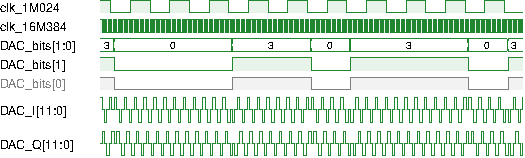
\includegraphics{_tikz_sim_Tx_BPSK-crop.pdf}}\\
        \subfloat[QPSK modulation.]{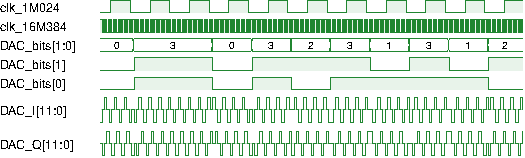
\includegraphics{_tikz_sim_Tx_QPSK-crop.pdf}}
        \caption{DAC simulation results of the transmitter.
          The gray line denotes the wave is irrelevant.
          The DAC waveforms are displayed in the \textit{hold} mode, in contrast to the \textit{linear} mode.}
        \label{fig:tx_dac_sim}
      \end{figure}

      Due to the limited number of samples (4 per period), the DAC output is not smooth, and shapes like a triangle wave.
      Nevertheless, the phase shift for both I and Q at symbol transitions is clear.

    \subsection{Carrier Synchronization Convergence}\label{subsec:costas_convergence}

      The simulation results of the Costas loop are shown in Fig.~\ref{fig:sync_BPSK}.
      The convergence is relatively fast.
      In the BPSK mode, the Costas loop can successfully handle the CFO smaller than \qty{7.81}{kHz}.
      It can be verified by the fact that the feedback saturates around a constant,
      which corresponds to the CFO value.
      In the QPSK mode, the threshold value is \qty{1.96}{kHz}.
      \begin{figure}[htbp]
        \centering
        % \begin{tikzpicture}
  \begin{axis}[
    , semithick
    , enlarge x limits = false
    , width = \linewidth
    , height = .7\linewidth
    , grid = both
    , legend style = {
      , font = \notsotiny
      , cells = {
        , align = right
        , anchor = east
        , line width = 1pt
      }
    }
    , legend columns=2
    , scaled x ticks = false
    , xtick = {2048, 2048+1024, 2048+1024*2, 2048+1024*3, 2048+1024*4, 2048+1024*5, 2048+1024*6, 2048+1024*7, 2048+1024*8}
    , xticklabels = {0, 256, 512, 768, 1024, 1280, 1635, 1792, 2048}
    , ylabel near ticks
    , xlabel near ticks
    , label style = { font = \scriptsize, inner sep = 0pt }
    , tick label style = {font = \notsotiny }
    , ylabel = {Feedback}
    , xlabel = {Clock}
    , xmin = 4 * 512
    , xmax = 20 * 512
    , ymin = -100
    , ymax = 100
  ]
    \addplot [
      , color = myred
      , opacity = .8
      , mark = none
    ] table [
      , col sep = comma
      , skip first n = 420
    ] {../behav_sim/BPSK_behav_sim_-32_F.csv};

    \addplot [
      , color = myblued
      , opacity = .8
      , mark = none
    ] table [
      , col sep = comma
      , skip first n = 420
    ] {../behav_sim/BPSK_behav_sim_-16_S0.csv};

    \addplot [
      , color = mygreen
      , opacity = .8
      , mark = none
    ] table [
      , col sep = comma
      , skip first n = 420
    ] {../behav_sim/BPSK_behav_sim_-8_S0.csv};

    \addplot [
      , color = myyellow
      , opacity = .8
      , mark = none
    ] table [
      , col sep = comma
      , skip first n = 420
    ] {../behav_sim/BPSK_behav_sim_+8_S1.csv};

    \addplot [
      , color = mypurple
      , opacity = .8
      , mark = none
    ] table [
      , col sep = comma
      , skip first n = 420
    ] {../behav_sim/BPSK_behav_sim_+16_S1.csv};

    \addplot [
      , color = gray
      , opacity = .8
      , mark = none
    ] table [
      , col sep = comma
      , skip first n = 420
    ] {../behav_sim/BPSK_behav_sim_+32_F.csv};

    \legend{
      $\qty[retain-explicit-plus]{-15.6}{kHz}$,
      $\qty[retain-explicit-plus]{-7.81}{kHz}$,
      $\qty[retain-explicit-plus]{-3.91}{kHz}$,
      $\qty[retain-explicit-plus]{+3.91}{kHz}$,
      $\qty[retain-explicit-plus]{+7.81}{kHz}$,
      $\qty[retain-explicit-plus]{+15.6}{kHz}$,
    };
  \end{axis}
\end{tikzpicture}%

        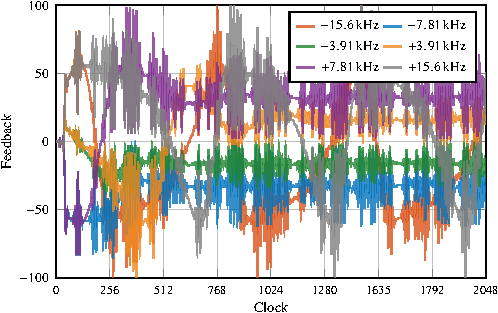
\includegraphics{_tikz_sim_sync_BPSK-crop.pdf}
        \caption{Carrier synchronization for BPSK. The feedback value after the loop filter v.s.\ time, with different CFO.}
        \label{fig:sync_BPSK}
      \end{figure}
      
      Notably, the convergence performance of QPSK is poorer than BPSK in the current parameter set,
      which is by design.
      For a dual-mode system which transmits payload in both BPSK and QPSK with a BPSK header,
      the carrier synchronization is achieved at the BPSK header.
      Therefore, QPSK does not need a strong feedback.
      Furthermore, a smaller feedback can make the BPSK and QPSK transition smoother,
      avoiding a sudden phase jump of $90^\circ$.

    \subsection{Mixed-Mode Receiver}

      \begin{figure*}
        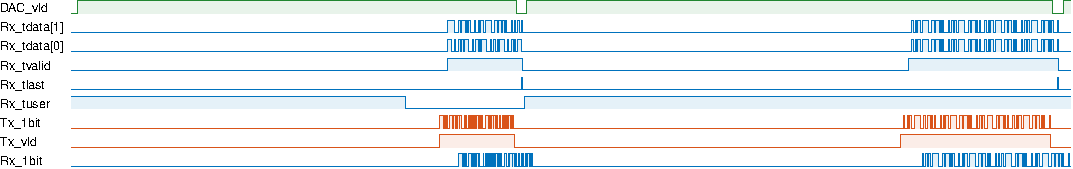
\includegraphics{_tikz_sim_MIX-crop.pdf}
        \caption{Mixed-mode simulation results.
          The first packet is transmitted using QPSK, and the second packet is transmitted using BPSK.}
        \label{fig:mix_sim}
      % \end{figure*}
      % \begin{figure*}[t]
        % \subfloat[BPSK packet data (duration: \qty{200}{\micro\second}).\label{subfig:scope_bpsk}]{\begin{tikzpicture}[
  , font = \sffamily
]
  \begin{axis}[
    , width = \linewidth
    , height = 10mm
    , scale only axis = true
    , enlarge x limits = false
    , axis line style = { draw = none }
    , ticks = none
    , thick
  ]
    \addplot [
      , color = myred
      , mark = none
    ] table [
      , col sep = comma
      , skip first n = 2
      , x index = 0
      , y index = 1
    ] {../scope/BPSK.csv};
    \addplot [
      , color = myblued
      , mark = none
      , y filter/.code = {\pgfmathparse{\pgfmathresult-45}}
    ] table [
      , col sep = comma
      , skip first n = 2
      , x index = 0
      , y index = 2
    ] {../scope/BPSK.csv};

    \node [anchor = north west, myred] at (rel axis cs:0,1) {Tx};
    \node [anchor = south west, myblued] at (rel axis cs:0,0) {Rx};
  \end{axis}
\end{tikzpicture}%
}\\
        % \subfloat[QPSK packet data (duration: \qty{100}{\micro\second}).\label{subfig:scope_qpsk}]{\begin{tikzpicture}[
  , font = \sffamily
]
  \begin{axis}[
    , width = \linewidth
    , height = 10mm
    , scale only axis = true
    , enlarge x limits = false
    , axis line style = { draw = none }
    , ticks = none
    , thick
  ]
    \addplot [
      , color = myred
      , mark = none
    ] table [
      , col sep = comma
      , skip first n = 2
      , x index = 0
      , y index = 1
    ] {../scope/QPSK.csv};
    \addplot [
      , color = myblued
      , mark = none
      , y filter/.code = {\pgfmathparse{\pgfmathresult-45}}
    ] table [
      , col sep = comma
      , skip first n = 2
      , x index = 0
      , y index = 2
    ] {../scope/QPSK.csv};

    \node [anchor = north west, myred] at (rel axis cs:0,1) {Tx};
    \node [anchor = south west, myblued] at (rel axis cs:0,0) {Rx};
  \end{axis}
\end{tikzpicture}%
}\\
        % \subfloat[Symbol timing clock and BPSK data at Rx (duration: \qty{50}{\micro\second}).\label{subfig:scope_timing}]{\begin{tikzpicture}[
  , font = \sffamily
]
  \begin{axis}[
    , width = \linewidth
    , height = 7.5mm
    , scale only axis = true
    , enlarge x limits = false
    , axis line style = { draw = none }
    , ticks = none
    , thick
  ]
    \addplot [
      , color = myred
      , mark = none
    ] table [
      , col sep = comma
      , skip first n = 2
      , x index = 0
      , y index = 1
    ] {../scope/timing_BPSK.csv};
    \addplot [
      , color = myblued
      , mark = none
      , y filter/.code = {\pgfmathparse{\pgfmathresult-45}}
    ] table [
      , col sep = comma
      , skip first n = 2
      , x index = 0
      , y index = 2
    ] {../scope/timing_BPSK.csv};

    \node [anchor = south east, myblued] at (rel axis cs:1,0) (data) {Rx Data};
    \node [left = 2mm of data, myred, yshift = 1mm] {Rx Clk.};
  \end{axis}
\end{tikzpicture}%
}
        \subfloat[BPSK packet data (duration: \qty{200}{\micro\second}).\label{subfig:scope_bpsk}]{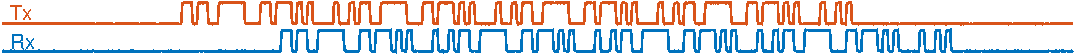
\includegraphics{_tikz_scope_BPSK-crop.pdf}}\\
        \subfloat[QPSK packet data (duration: \qty{100}{\micro\second}).\label{subfig:scope_qpsk}]{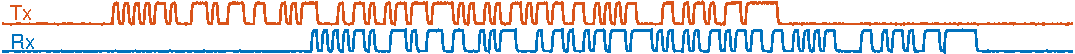
\includegraphics{_tikz_scope_QPSK-crop.pdf}}\\
        \subfloat[Symbol timing clock and BPSK data at Rx (duration: \qty{50}{\micro\second}).\label{subfig:scope_timing}]{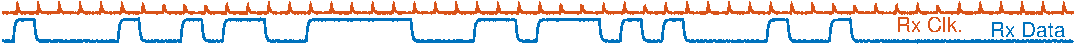
\includegraphics{_tikz_scope_timing-crop.pdf}}
        \caption{Two-channel oscilloscope results of GPIO outputs.}
        \label{fig:scope}
      \end{figure*}

      In this simulation, we show the successful transmission of packets in both BPSK and QPSK modulations.
      The simulation results are shown in Fig.~\ref{fig:mix_sim}.

      The DAC transmits data when \texttt{DAC\_vld} is high,
      and the payload is transmitted when \texttt{Tx\_vld} is high.
      There is a delay of 
      The two packet streams are clearly shown,
      with the first being QPSK and the second being BPSK, both of 128 bits length.
      The \texttt{Rx\_tuser} signal shows the detected modulation scheme at the Rx, with 1 for BPSK and 0 for QPSK.
      Since QPSk has a $2\times$ bit rate, the first packet payload is transmitted $2\times$ faster than the first one.

  \section{FPGA Implementation}

    The design is implemented in Vivado 2022.2 using block diagrams.
    Some block diagram designs are shown in Section~\ref{sec:block_diagrams}.

    The hardware resources consumption on the Zynq-7020 (xc7z020clg484-1) board
    with the default synthesis and implementation strategy is shown in Table~\ref{tab:resource}.
    Therefore, the design itself is resource-efficient, and can be readily incorporated into a larger system.
    \begin{table}[htbp]
      \caption{Hardware Resources Consumption on Zynq-7020}
      \label{tab:resource}
      \renewcommand{\arraystretch}{1.2}
      \rowcolors{1}{white}{gray!15}
      \begin{tabularx}{\linewidth}{YYYY}
        \toprule\tabvertspace
        \textbf{Resource} & \textbf{Utilization} & \textbf{Available} & \textbf{Util.\ Rate} \\
        \tabvertspace\midrule
        LUT & 7,248 & 53,200 & \hphantom{0}8.04\% \\
        LUTRAM & 1,121 & 17,400 & \hphantom{0}6.44\% \\
        FF & 8,144 & 106,400\hphantom{0} & \hphantom{0}7.65\% \\
        BRAM & \hphantom{0,0}27 & \hphantom{00,}140 & 19.29\% \\
        DSP & \hphantom{0,0}51 & \hphantom{00,}220 & 23.18\% \\
        IO & \hphantom{0,0}33 & \hphantom{00,}200 & 16.50\% \\
        BUFG & \hphantom{0,0}10 & \hphantom{00,0}32 & 31.25\% \\
        MMCM & \hphantom{0,00}2 & \hphantom{00,00}4 & 50.00\% \\
        \bottomrule
      \end{tabularx}
    \end{table}

    The FPGA design source is open source \cite{github_repo},
    and parts of the design can be easily reused in other projects.

  \section{Experiment Results on SDR}

    The eNodeX SDR platform \cite{eNodeX} is configured to provide 1 Tx and 1 Rx
    at a sampling frequency of \qty{16.384}{MHz}.
    The GSM antenna carrier frequency is \qty{800}{MHz},
    and the two antennas have a line-of-sight (LoS) channel.

    The parameters used in this design
    are specially adjusted for received signal with strength ranging between $1/2$ and $3/4$ of the full ADC range.
    Therefore, you should adapt the antenna attenuation and gains to get the appropriate signal strength.
    With AD9361 \cite{ad9361},
    each ADC stream has 12 bits as a signed number, i.e., ranging between $-2048$ and $2047$.

    The experiment results are observed via a system ILA in Vivado,
    and 4 general-purpose input/output (GPIO) pins are used to output some 1-bit signals,
    including the 1-bit Tx and Rx data stream and their corresponding clock.

    In our design, 4 GPIO pins are connected, as listed in Table~\ref{tab:gpio_pins}.
    Fig.~\ref{fig:scope} shows the oscilloscope results of the GPIO outputs.
    \begin{table}[htbp]
      \caption{GPIO Pin Connections}
      \label{tab:gpio_pins}
      \renewcommand{\arraystretch}{1.2}
      \rowcolors{1}{white}{gray!15}
      \begin{tabularx}{\linewidth}{cX}
        \toprule\tabvertspace
        \textbf{Pin} & \textbf{Signal} \\
        \tabvertspace\midrule
        \texttt{GPIO\_TH1} & Tx 1-bit sequence (clock: \qty{1.024}{MHz} or \qty{2.048}{MHz}) \\
        \texttt{GPIO\_TH2} & Rx 1-bit sequence (sync.\ w/ Rx timing clock when BPSK) \\
        \texttt{GPIO\_TH3} & \qty{2.048}{MHz} global clock from the clock divider \\
        \texttt{GPIO\_TH4} & Rx timing clock ($\sim$\qty{1.024}{MHz}) \\
        \bottomrule
      \end{tabularx}
    \end{table}

    In Fig.~\subref*{subfig:scope_bpsk} and Fig.~\subref*{subfig:scope_qpsk},
    the \texttt{GPIO\_TH1} and \texttt{GPIO\_TH2} pins are connected,
    showing the transmitted 1-bit sequence (Tx) and the respective received 1-bit sequence (Rx).
    Clearly, the sequence is successfully recovered in both cases, with a certain time delay.
    The structure of \texttt{pn\_5} sequence in BPSK is clearly seen in Fig.~\subref*{subfig:scope_bpsk},
    which has a bit frequency of \qty{1.024}{MHz}.
    By contrast, the bit frequency of QPSK packets in Fig.~\subref*{subfig:scope_qpsk} is \qty{2.048}{MHz}.
    The symbol timing clock is shown in Fig.~\subref*{subfig:scope_timing},
    which is not synchronized with the Rx data in BPSK,
    as the Rx data is connected after a FIFO with the master clock of \qty{1.024}{MHz}.
    The symbol timing clock has a measured frequency of near \qty{1.024}{MHz} on the oscilloscope.

    % \begin{figure*}[t]
    %   % \subfloat[BPSK packet data (duration: \qty{200}{\micro\second}).\label{subfig:scope_bpsk}]{\begin{tikzpicture}[
  , font = \sffamily
]
  \begin{axis}[
    , width = \linewidth
    , height = 10mm
    , scale only axis = true
    , enlarge x limits = false
    , axis line style = { draw = none }
    , ticks = none
    , thick
  ]
    \addplot [
      , color = myred
      , mark = none
    ] table [
      , col sep = comma
      , skip first n = 2
      , x index = 0
      , y index = 1
    ] {../scope/BPSK.csv};
    \addplot [
      , color = myblued
      , mark = none
      , y filter/.code = {\pgfmathparse{\pgfmathresult-45}}
    ] table [
      , col sep = comma
      , skip first n = 2
      , x index = 0
      , y index = 2
    ] {../scope/BPSK.csv};

    \node [anchor = north west, myred] at (rel axis cs:0,1) {Tx};
    \node [anchor = south west, myblued] at (rel axis cs:0,0) {Rx};
  \end{axis}
\end{tikzpicture}%
}\\
    %   % \subfloat[QPSK packet data (duration: \qty{100}{\micro\second}).\label{subfig:scope_qpsk}]{\begin{tikzpicture}[
  , font = \sffamily
]
  \begin{axis}[
    , width = \linewidth
    , height = 10mm
    , scale only axis = true
    , enlarge x limits = false
    , axis line style = { draw = none }
    , ticks = none
    , thick
  ]
    \addplot [
      , color = myred
      , mark = none
    ] table [
      , col sep = comma
      , skip first n = 2
      , x index = 0
      , y index = 1
    ] {../scope/QPSK.csv};
    \addplot [
      , color = myblued
      , mark = none
      , y filter/.code = {\pgfmathparse{\pgfmathresult-45}}
    ] table [
      , col sep = comma
      , skip first n = 2
      , x index = 0
      , y index = 2
    ] {../scope/QPSK.csv};

    \node [anchor = north west, myred] at (rel axis cs:0,1) {Tx};
    \node [anchor = south west, myblued] at (rel axis cs:0,0) {Rx};
  \end{axis}
\end{tikzpicture}%
}\\
    %   % \subfloat[Symbol timing clock and BPSK data at Rx (duration: \qty{50}{\micro\second}).\label{subfig:scope_timing}]{\begin{tikzpicture}[
  , font = \sffamily
]
  \begin{axis}[
    , width = \linewidth
    , height = 7.5mm
    , scale only axis = true
    , enlarge x limits = false
    , axis line style = { draw = none }
    , ticks = none
    , thick
  ]
    \addplot [
      , color = myred
      , mark = none
    ] table [
      , col sep = comma
      , skip first n = 2
      , x index = 0
      , y index = 1
    ] {../scope/timing_BPSK.csv};
    \addplot [
      , color = myblued
      , mark = none
      , y filter/.code = {\pgfmathparse{\pgfmathresult-45}}
    ] table [
      , col sep = comma
      , skip first n = 2
      , x index = 0
      , y index = 2
    ] {../scope/timing_BPSK.csv};

    \node [anchor = south east, myblued] at (rel axis cs:1,0) (data) {Rx Data};
    \node [left = 2mm of data, myred, yshift = 1mm] {Rx Clk.};
  \end{axis}
\end{tikzpicture}%
}
    %   \subfloat[BPSK packet data (duration: \qty{200}{\micro\second}).\label{subfig:scope_bpsk}]{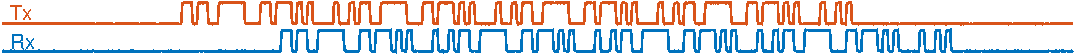
\includegraphics{_tikz_scope_BPSK-crop.pdf}}\\
    %   \subfloat[QPSK packet data (duration: \qty{100}{\micro\second}).\label{subfig:scope_qpsk}]{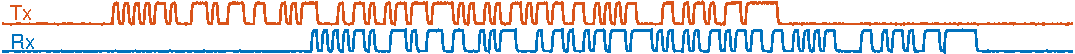
\includegraphics{_tikz_scope_QPSK-crop.pdf}}\\
    %   \subfloat[Symbol timing clock and BPSK data at Rx (duration: \qty{50}{\micro\second}).\label{subfig:scope_timing}]{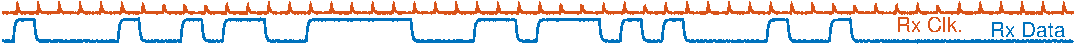
\includegraphics{_tikz_scope_timing-crop.pdf}}
    %   \caption{Two-channel oscilloscope results of GPIO outputs.}
    %   \label{fig:scope}
    % \end{figure*}

    Fig.~\ref{fig:ila} gives the ILA results for two cases involving BPSK and QPSK.
    The ILA results are consistent with the oscilloscope results,
    and provide additional insight into the system, including PSK detection and packet extraction.
    The \texttt{I\_16M} and the \texttt{Q\_16M} signals are the I and Q components of the data stream signal from the Costas loop,
    while the \texttt{I\_1M} and the \texttt{Q\_1M} signals are provided by the Gardner loop after symbol timing.
    The \texttt{out\_clk\_1M} clock is the symbol timing clock, which is near optimal, as designed by the Gardner loop.

    \begin{figure*}[!t]
      \setlength{\tabcolsep}{2pt}
      \subfloat[A BPSK packet (with \textsf{Rx\_data\_tuser} high).]{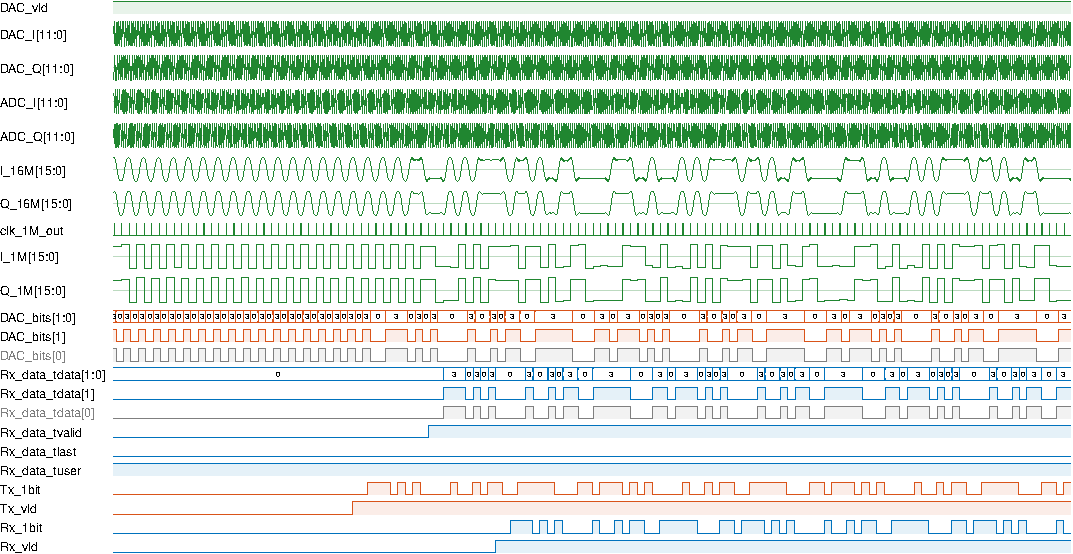
\includegraphics{_tikz_ila_BPSK-crop.pdf}}\\
      \subfloat[A QPSK packet (with \textsf{Rx\_data\_tuser} low).]{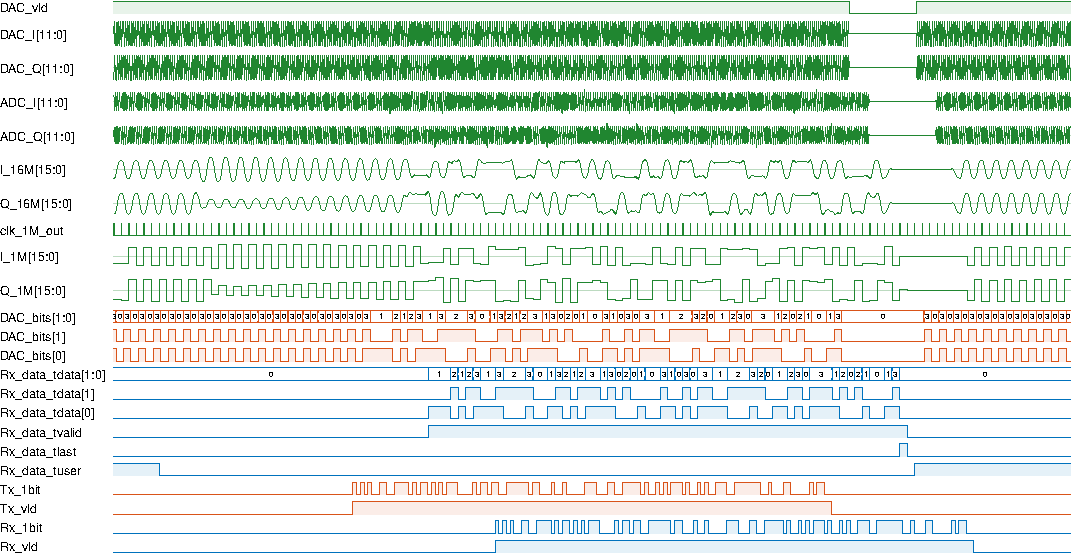
\includegraphics{_tikz_ila_QPSK-crop.pdf}}\\
      \caption{System ILA results (some signals not shown, and this is plotted with the saved CSV data).
        The system ILA has a window of 4,096, with the ILA clock frequency of \qty{32.768}{MHz} (twice the ADC/DAC sampling rate).
        The \textcolor{myred}{red} and \textcolor{myblued}{blue} signals are at the Tx and Rx side, respectively.
        }
      \label{fig:ila}
    \end{figure*}

  \section{Discussions}

    \subsection{Possible Enhancement}

      \textbf{Frame structure design}.
      CRC and/or checksums can be added to the frame structure to enhance the packet transmission stability in Section~\ref{subsec:frame_structure}.
      Additionally,
      the HDR and TRN field in Section~\ref{subsec:frame_structure} may have some improvements.
      The Golay sequence used in \cite{IEEE802.11ad,lacruz2021real,zhao2023automatic} is one possible better solution:
      it has a better performance at low SNR, and the packet detection based on autocorrelation \cite{lacruz2021real}
      can reduce power consumption by disabling the demodulation when there is no packet.

      \textbf{Changing parameters on the fly}.
      AXI peripheral \cite{xilinx:pg127} can be used to change the parameters in the \texttt{Const\_Config} on the fly,
      if the board allows.
      Therefore, the BPSK/QPSK/mixed mode can be switched directly,
      and the parameters in the design can be changed without recompiling the design,
      allowing easier use in various scenarios.

      \textbf{Pulse shaping}.
      The SNR performance will be improved if appropriate pulse shaping is employed.
      This enhancement is left as an exercise for the reader.

    \subsection{Possible Extensions Beyond the Experiment}

      The training (TRN) field can be better utilized for additional experiments.
      For example, SNR can be estimated at the TRN field,
      so a plot with BER against SNR can be obtained.
      Channel estimation algorithms \cite{zhao2023ompl,you2023beam} can also be investigated on the platform,
      allowing the test of the performance of the algorithms in real-world scenarios.
      Besides, it is also possible to investigate the auto generation \cite{zhao2023automatic} of digital circuits,
      so that the design can be automatically generated according to different requirements.

  \section{Conclusion}

    In this paper,
    we implement the PSK transceiver with modulation and coherent demodulation on SDR with FPGA.
    The proposed high-level system design and communication techniques
    feature carrier synchronization, symbol synchronization and packet-based communication.
    The design is tested and verified on a SDR platform, successfully performing wireless transmission in \qty{2.048}{Mb/s} data rate using QPSK
    or \qty{1.024}{Mb/s} data rate using BPSK
    with a \qty{16.384}{MHz} bandwidth (considering I/Q sampling) channel.
    As an open source project,
    this paper opens up new possibilities of easy extension of the PSK transceiver.

  \appendices

  \begin{figure*}[!t]
    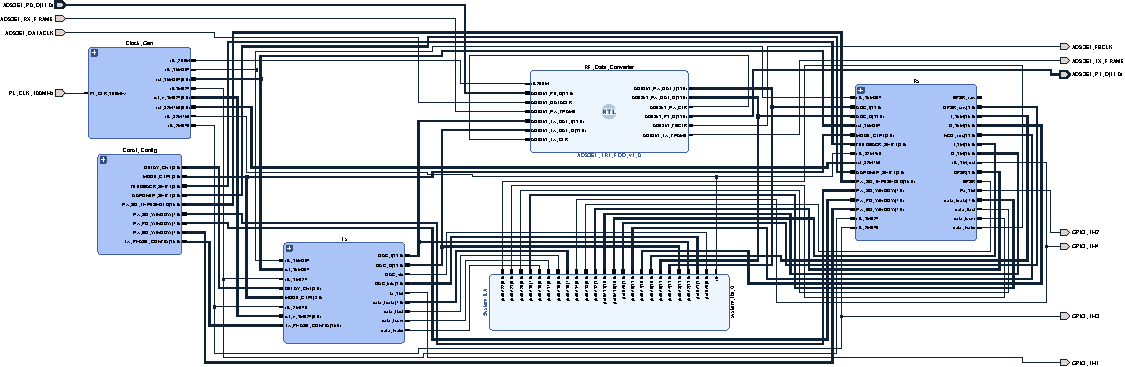
\includegraphics[width=\linewidth]{../schematic/top.pdf}
    \caption{Top block diagram.}
    \label{fig:block_top}
    \vspace*{.5em}
  % \end{figure*}
  % \begin{figure*}
    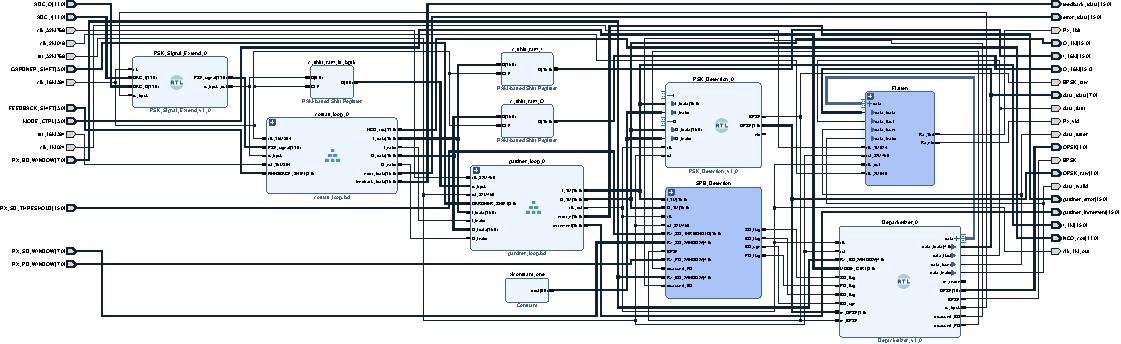
\includegraphics[width=\linewidth]{../schematic/Rx.pdf}
    \caption{Rx processor block diagram.}
    \label{fig:block_rx}
  % \end{figure*}
  % \begin{figure*}
    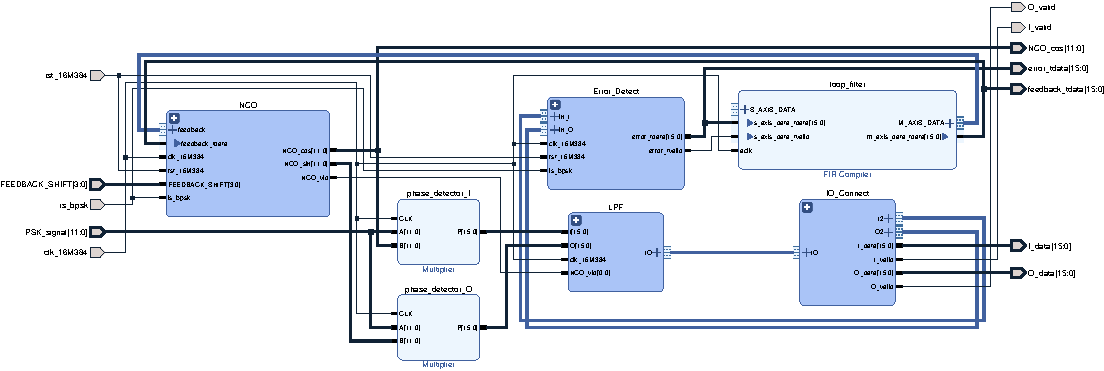
\includegraphics[width=\linewidth]{../schematic/costas_loop.pdf}
    \caption{Costas loop block diagram for carrier synchronization.}
    \label{fig:block_costas_looop}
  \end{figure*}

  \section{Block Diagrams}\label{sec:block_diagrams}

    \subsection{Block Diagrams Design}

    The top level block diagram corresponding to Fig.~\ref{fig:system_overview} is shown in Fig.~\ref{fig:block_top},
    and the Rx processor block diagram is shown in Fig.~\ref{fig:block_rx}.
    Among the Rx processor, the Costas loop and the Gardner are both inserted block diagrams.

    The Costas loop design is shown in Fig.~\ref{fig:block_costas_looop},
    where the phase detectors are implemented using the multiplier IP \cite{xilinx:pg108},
    and the NCO hierarchy is mainly composed of the DDS Compiler IP \cite{xilinx:pg141}.
    The LPF hierarchy contains a low-pass filter with 2 channels (I and Q).

    More block diagrams are provided at \url{https://github.com/Teddy-van-Jerry/sdr-psk-fpga/tree/master/schematic} \cite{github_repo}.

    \subsection{Debugging With Block Diagrams}

      \textbf{AXI connections}.
      AXI and AXI stream (AXIS) interfaces should be carefully dealt with in the block diagram.
      When connecting one of the signal in the bus elsewhere (e.g., to ILA),
      a manual connection of the signal to the corresponding AXIS interface signal is required.
      Besides, when the AXI interface is not associated with a clock (for example a combinational logic with no register output)
      the \texttt{FREQ\_HZ} property needs to be correctly set (either using Tcl or GUI) before validating the design.

      \textbf{Testbenches for block diagrams}.
      It is relatively difficult to simulate block diagrams than Verilog modules.
      The possible way is to generate the output products and find the correct module (name containing \texttt{impl}).
      Be careful when adding sources for simulation, and Tcl scripts are provided in \cite{github_repo} to ensure the correctness.
      Vivado can be buggy (mostly reluctant!) when updating sources from the block diagram (for both simulation and implementation),
      and therefore it is advised to double-check the netlist file timestamp.
      A workaround by forcing Vivado to update the design is adding a dummy port, updating the module, and then removing it.

      \textbf{Suggestions}.
      The project could have been more smooth if I did without block diagrams (or for AMD to fix all these bugs).
      You can directly use the Verilog modules in \cite{github_repo} for your own project if you are not accustomed to block diagrams.
      Nevertheless, block diagrams are at least better looking and easier to use for a system-level project,
      especially when dealing with the system on a chip (SoC).


  \section{Figures in This Paper}

    All figures except for block diagrams in this paper
    are created using T\textit{i}kZ, part of \LaTeX{}.
    The way I create them is quite interesting, involving extensive Python processing and optimization,
    and you can find the source code in the GitHub repository \cite{github_repo}.

  \bibliographystyle{IEEEtran}
  \bibliography{IEEEabrv, ref}

  \begin{IEEEbiographynophoto}%
    {Wuqiong Zhao} (S'22)
    is a senior undergraduate student pursuing the Bachelor's Degree in communications engineering,
    at the National Mobile Communications Research Laboratory of Southeast University, Nanjing, China.
    His research interests include wireless systems and networking, signal processing, and hardware implementation.
    He has published several journal papers at \textsc{IEEE Transactions on Vehicular Technology} (TVT)
    and \textsc{IEEE Transactions on Circuits and Systems II} (TCAS-II).
    He was also reviewers of IEEE ISCAS 2023 and IEEE TCAS-II.
    Visit the website \url{https://wqzhao.org} for more information.
  \end{IEEEbiographynophoto}

\end{document}
